\chapter{Введение}
Образовательные технологии --- это важно потому, что рыба рыба рыба рыба рыба рыба рыба рыба.

Автоматизация --- это важно потому, что рыба рыба рыба рыба рыба рыба рыба рыба рыба рыба.

Робототехника --- это важно потому, что рыба рыба рыба рыба рыба рыба рыба рыба рыба рыба.
\section{актуальность работы}
Исследование употребления в СМИ образовательных технологий и робототехники. 

\begin{figure}[ht]
    \centering
    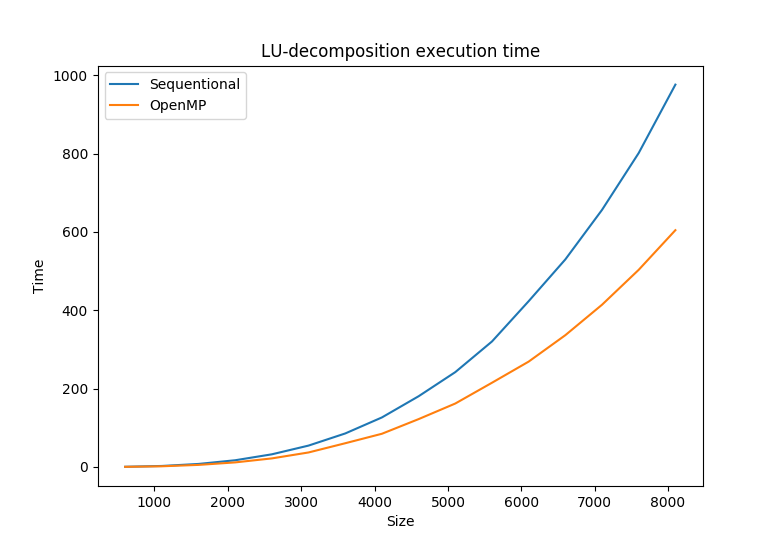
\includegraphics[scale=0.7]{../images/mock1.png}
    \caption{заглушка}
\end{figure}

Популярные подходы к автоматизации образовательного процесса и их общий недостаток. Возникает задача найти подход, лишённый этот недостаток.
\section{значимость работы}
Робототехнический подход, основанный на реактивно"=делиберативном подходе, решает поставленную выше задачу, также у него есть иные плюсы.

\section{объект работы}
\textbf{Объект работы} -- когнитивный робот как единица образовательной робототехники.

\section{предмет работы}
\textbf{Предмет работы} --- реактивно"=делиберативный подход к созданию когнитивных роботов.

\section{цель работы}
\textbf{Цель работы} --- разработка программно"=аппаратного комплекса для создания диалоговых когнитивных роботов на основе реактивно"=делиберативного подхода.
